\section{Coletas de Dados com os Pacientes}

% ********************** FALAR DO COMITE DE ÉTICA *************************  
% - TAMANHO DA AMOSTRAGEM / LOCAL DE COLETA - Falar do LIS / falar da especialista / explicitar que esta fase vai para dentro do software / Acrescentar anexo (ficha, tcle) e apendice (doc visao e arquitetura) / 

    As coletas de dados foram implementadas seguindo uma estrutura de ficha, definida a partir das normas de avaliação CIF. Sendo assim, todas as coletas de dados seguiram a ordem conforme a Figura 7. 

    \begin{itemize}
        \item Acolhimento do paciente e coleta de seus dados pessoais;
        \item Aplicação da ficha de avaliação do paciente, feita por um profissional da área de saúde;
        \item Sessão de fotos do coto e do paciente para futura análise postural e de condição da pele.
    \end{itemize}

    A ficha de avaliação aplicada junto ao paciente pelo profissional da saúde é um dos produtos de software desenvolvidos para facilitar e agilizar a avaliação do paciente.

    \begin{figure}[ht]
        \centering
        \label{fig07}
            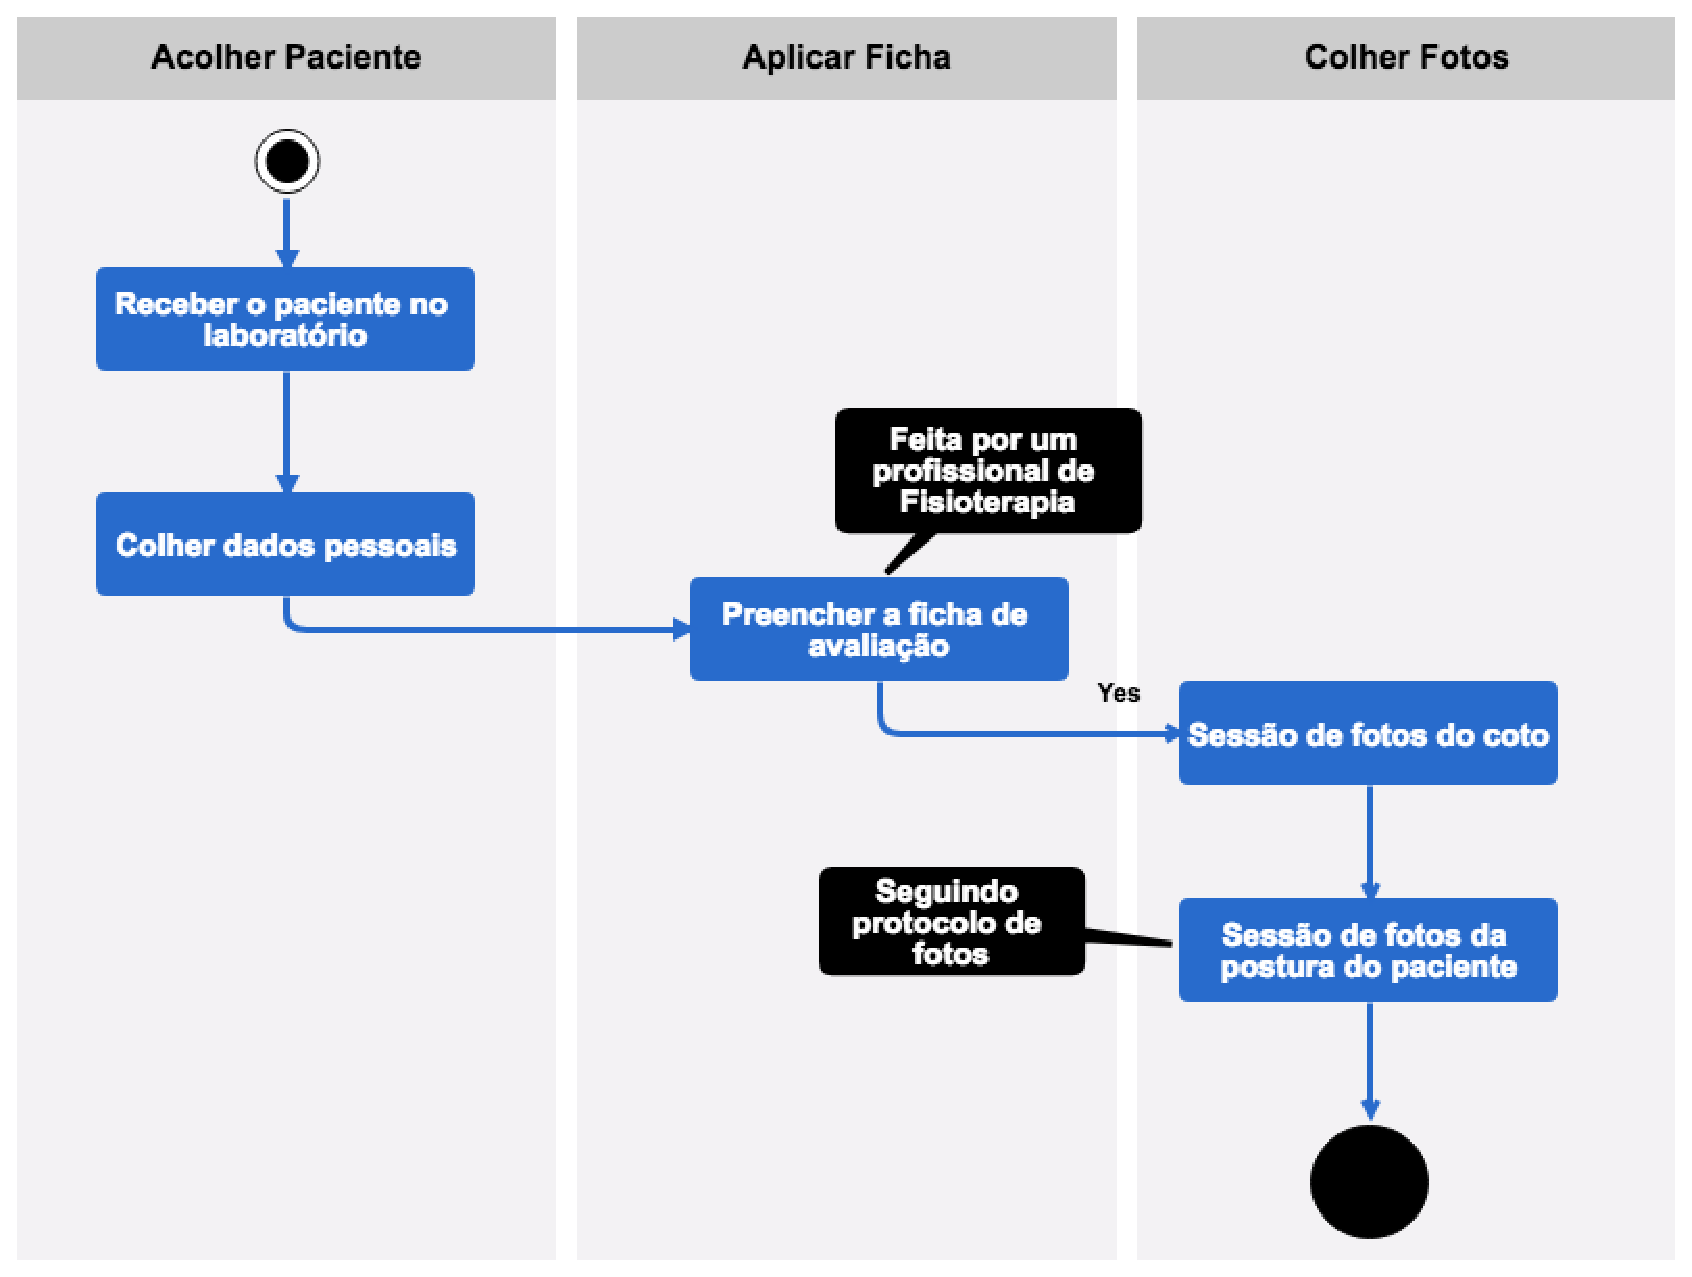
\includegraphics[keepaspectratio=true, scale=0.4]{editaveis/images/colet_flow.eps}
        \caption{Fluxo de trabalho da coleta}
    \end{figure}

    A sessão de fotos do coto do paciente, foi pensada para ser o mais simples possível, para que todo profissional da área da saúde possa conseguir coletar este dado sem necessidade de conhecimento técnico de fotografia ou de um protocólo rígido. O profissional da saúde precisará apenas de uma câmera fotográfica, ou celular com câmera, para fazer o registro com a única restrição de que a imagem gerada seja completamente preenchida pela pele do paciente.

    Para que pudessem ser feitas as coletas de dados de pacientes, é necessário um Comitê de Ética, o qual disponibilizou a autorização com o número CAAE 38386714.8.0000.0030. Foram feitas coletas com 13 pacientes diferentes no decorrer da pesquisa, todas com o auxílio de uma fisioterapeuta especialísta na área de tratamento com pacientes amputados.

    Os dados foram coletados em sua maioria no Laboratório de Análise de Movimento e Processamento de Sinais da Faculdade da Ceilândia da Universidade de Brasília (FCE-UnB), a pesar de terem ocorrido casos em que a coleta foi feita na casa do paciente, trabalhando em conjunto com o centro da pesquisa que foi o Laboratório de Informática e Saúde (LIS) da Faculdade do Gama da Universidade de Brasília (FGA-UnB). 


    % \begin{figure}[ht]
    %     \centering
    %     \label{fig08}
    %         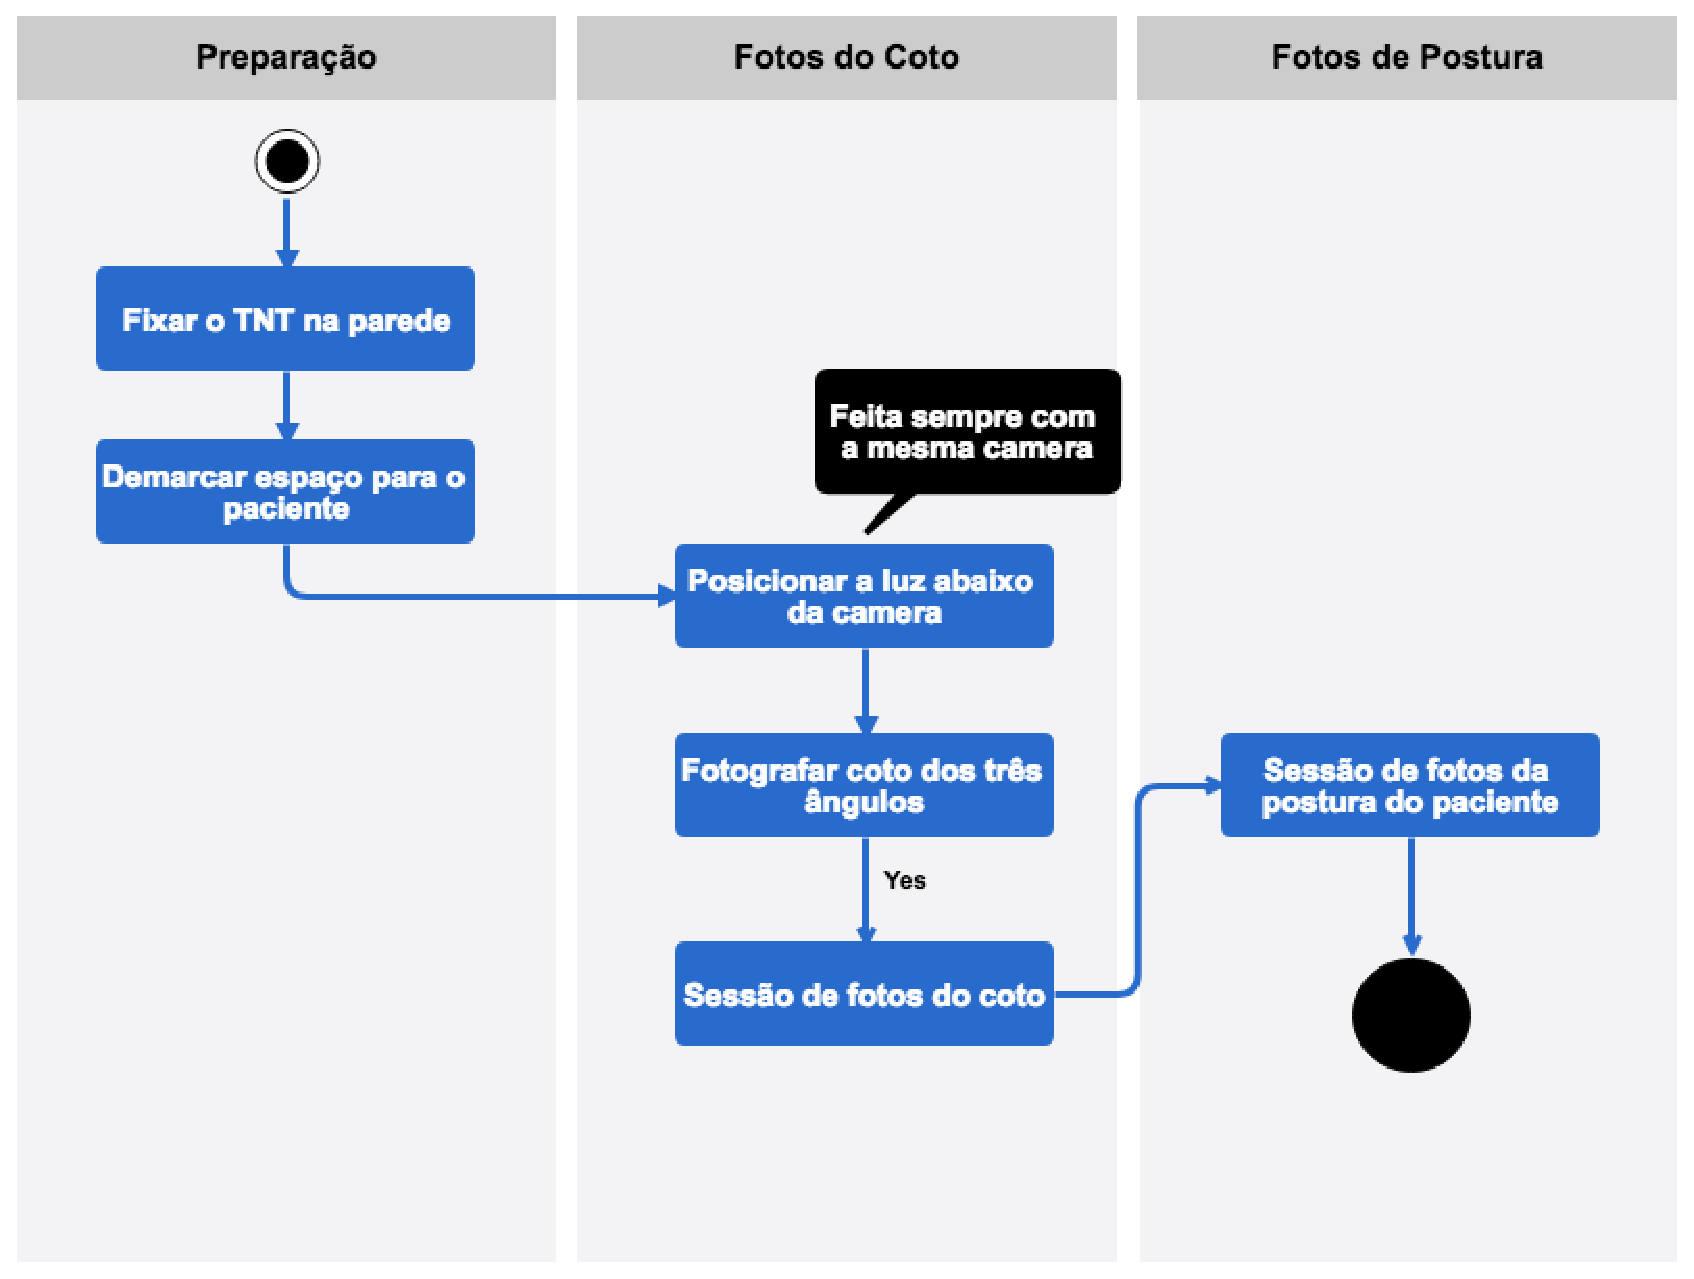
\includegraphics[keepaspectratio=true, scale=0.4]{editaveis/images/fotos_flow.eps}
    %     \caption{Fluxo de trabalho das fotografias}
    % \end{figure}

\section{Software GPSATWeb}
    % ******************** DESCREVER SIGLA GPSAT **********************
    O \textit{software} GPSATWeb foi construído utilizando a interação de dois sistemas separados, um \textit{web} para interação com o usuário e uma api \textit{restful} que trabalha com as requisições de todos os dados do sistema. 

    \subsection{API Restful}

        ** Mudar arquitetura REST para fundamentação **
        A \textit{api} construída é um serviço \textit{web restul} construído para receber e transmitir os dados do sistema GPSATWeb via requisições remotas, pois assim o acesso à base de dados independe de o sistema estar \textit{online} ou não. O termo \textit{Representational State Transfer} (REST), define um conjunto de principios arquiteturais que podem ser usados para projetar serviços \textit{web} que trabalham com os recursos de algum sistema. Este tipo de arquitetura permite que se desenhe como os recursos de um sistema serão endereçados e transferido via requisições Hypertext Transfer Protocol, ou Protocolo de Transferência de Hipertexto (HTTP) \cite{Rodriguez2008}. O HTTP é um protocolo baseado em documentos, no qual uma requisição é um envelope com um documento enviado a um servidor ou aplicação. Este documento normalmente pode conter qualquer informação, porém existem alguns pontos que devem ser explícitos, tais como o método, um endereço e os \textit{headres}, que são as palavras chaves da requisição \cite{Masse2011}.

        Desta maneira, atravez das requisições HTTP, o sistema \textit{web} se comunica com a \textit{api} utilizando os métodos padrões HTTP \textit{post}, \textit{delete}, \textit{get} e \textit{put} \cite{Rodriguez2008}, os quais qualificam a ação a ser desencolvida sobre os dados pela \textit{api}. O método \textit{post} faz a \textit{api} receber novos dados e armazenar na base de dados, já o \textit{delete} faz com que ela delete os dados segundo um identificador do dado a ser deletado. Já os métodos \textit{get} e \textit{put} são utilizados para envio de dados ou atualização de dados respectivamente, visto que o método \textit{put} também pode ser utilizado para armazenar novos dados, mas por um padrão deste projeto está sendo utilizado somente para atualização de dados.

        A \textit{api} utiliza para a base de dados o MongoDb que é uma ferramenta de banco de dados orientado a documentos. Estes tipos de bancos de dados foram originalmente desenvolvidos para salvar documentos de todos os tipos, estes documentos são codificados em formatos padrões internacionais, tais como JSON ou XML. Suas vantagens, além da flexibilidade adiquirida por usar estes formatos, são segundo \cite{Moniruzzaman2013}:
            \begin{itemize}
                \item Baixa latência de resposta para leitura e escrita;
                \item Eficiência em armazenar grandes quantidades de dados;
                \item Alta escalabilidade.
            \end{itemize}
        

    \subsection{Web}
        O \textit{software} GPSATWeb foi construído utilizando a linguagem de programação Python e o \textit{framework} Django. Este \textit{framework} implementa o padrão de arquitetura \textit{Model-View-Controller} (MVC).

        O padrão de arquitetura MVC é dividido em três camadas: modelo, visão e controlador. Cada uma destas camadas é responsável por uma atividade dentro do sistema. Quais, sejam \cite{Lemos2013}:
            \begin{itemize}
                \item Modelo: Camada em que acontece a presistência dos dados do sistema em uma base de dados. Somente nesta camada as quatro operações básicas de um banco de dados, isto é, criação, edição, leitura e atualização de dados podem ocorrer;
                \item Visão: Camada de interação com o usuário. É nela que todos os dados sao mostrados e recebidos;
                \item Controlador: Camada que controla todo o fluxo do sistema. Nesta camada é feita a comunicação entre outras duas, a da visão e a de modelo. Além disso, nesta camada ocorre o processamento de todos os dados, tanto de entrada quanto de saída do sistema.
            \end{itemize}

        No caso do GPSATWeb, a camada modelo não interage diretamente com a base de dados, ela envia requisições HTTP com os dados a serem persistidos e o tipo de operação a ser realizada para a \textit{api}. 

    


\section{Modelo de Machine Learning}

    Tendo como meta a definição de um modelo de ML para ser aplicada em uma RNA a ser treinada para detecção de tipos de pele, a estratégia a ser seguida foi o fluxo de trabalho de ML, descrito na Figura 6 e adaptado para esta aplicação como mostra a Figura 9.

    \begin{figure}[ht]
        \centering
        \label{fig09}
            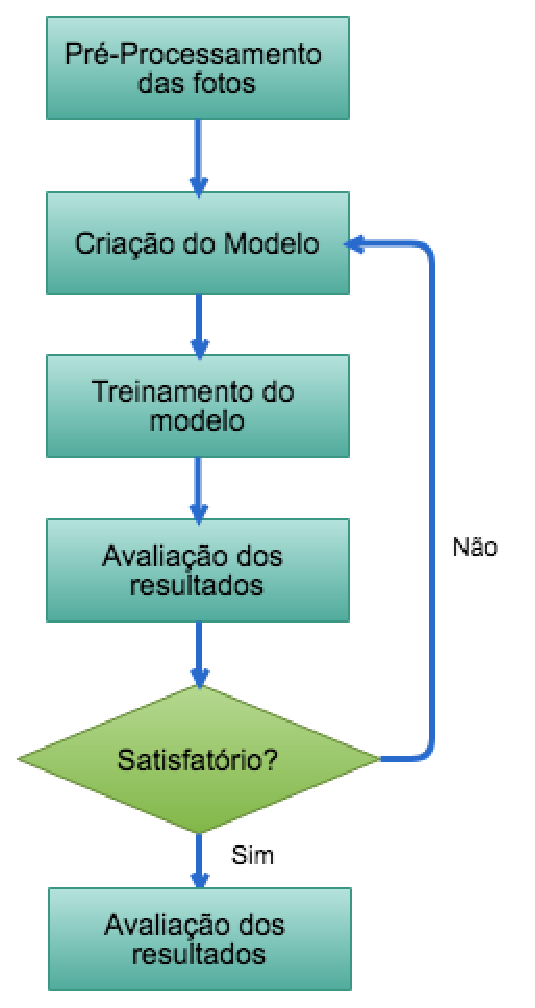
\includegraphics[keepaspectratio=true, scale=0.4]{editaveis/images/ml_nt_flow.eps}
        \caption{Fluxo de trabalho da construção do modelo de ML}
    \end{figure}

    \subsection{Construção do Modelo}

        O modelo de aprendizado utilizado é o supervisionado, baseado em uma RNA MLP com método de treinamento \textit{backpropagation}.
        Sendo assim, os passos a serem seguidos para a construção do modelo inicial são:

        \begin{itemize}
            \item Pré-processamento dos dados \\ Neste primeiro passo, é montado o modelo de dados de treinamento que será usado para apresentação e utilização dos dados. Para isso é necessário encontrar uma correlação entre os dados de entrada e o dado a ser atingido pelo processo de aprendizado.

            \item Criação do modelo \\ O modelo deve ser criado para receber os dados de entrada como pré-processados fazer seu processamento visando o resultado a ser obtido.

            \item Treinamento do modelo \\ O modelo proposto deve passar por um breve treinamento para que os erros sejam corrigidos antes que a rede comece a rebeber dados para serem analisados.

            \item Avaliar o modelo \\ Uma vez com o modelo pronto é necessário avaliar a aplicabilidade do modelo em vista da acurácia obtida em relação a quantidade de reconhecimentos feitos em uma base de dados controlada e com um número conhecido de dados coletados dos pacientes.

            \item Apresentar resultados \\ Assim que o modelo é avaliado, se for julgado com resultado insatisfatório, ele deve ser reencaminhado para uma melhoria na modelagem. Caso seja satisfatório, devem ser apresentados aqui os resultados obtidos.
        \end{itemize}
